\chapter{Evaluation}

\section{Experimental Results}
In order to avoid the degradation of KNN classification accuracy when the samples are unbalanced, we avoid using data from unbalanced samples in our tests. There is a case where the sample data contains only one category, then the KNN classification is meaningless, and the information loss is 0. After visualizing the data in Section 5, we see that the classification categories under bradykinesia disorders contain 'no,' 'yes,' and 'not applicable. There is a case where the sample data contains only one category, then the KNN classification is meaningless, and the information loss is 0. After visualizing the data in Section 5, we see that the classification categories under bradykinesia disorders contain 'no,' 'yes,' and 'not applicable. We filter the 'Notapplicate' points of bradykinesia and reclassify them, i.e., '0' and 'No' to the new '0' category and '1-4' to a new '1' category. So the classification categories under bradykinesia disorders are '0' and '1'. \\

A common task in machine learning is learning and predicting algorithms from data. \cite{RN3} Therefore, we divide the IMU dataset $X$ and the Parkinson's disease score dataset into a test set and a training set. The training set is used to train the model, and the test set is used to do the final evaluation. \cite{hastie2009elements}. When the model is trained, we cannot know how it will perform. We can use the validation set to see how the model performs on new data. The validation set has two purposes, 1. to evaluate the model and tune out the best k for testing KNN classification, and 2. to tune out the hyperparameters so that the model performs best on the validation set. Finally, we use the test set to compute our probability, $p(y|x)$. \cite{RN4} \\

We selected four patients with Parkinson's disease, i.e., patients 3, 6, 7, and 9. After getting the dataset, we will divide the dataset into a specific ratio. Our division ratio is 0.25; the test set is 0.25 of the dataset, and the training set is 0.75. We use the training set to build the KNN classification model and the test set to predict our probability $p(y|x)$. After getting the predicted probability $p(y|x)$, we bring in equation (6.1) and calculate the conditional entropy for each frequency. Once we have each conditional entropy, we calculate the difference between the conditional entropies at different sampling frequencies, the information loss. \\

First, we calculated the information loss on the left wrist of four patients under three conditions with decreasing sampling frequency. where the classification categories of tremor disorders were, '0', '1', '2', '3'. '4'. Dyskinesia disorders were classified in the categories '0', '1', '2', and bradykinesia disorders are classified in categories '0' and '1' as described above.\\
As in Figure 7.1, the blue, green, and orange lines correspond to the information loss with decreasing sampling frequency for dyskinesia, bradykinesia, and tremor disorders, respectively. We can see that the general trend of information loss is similar. Interestingly, the changes in information loss with decreasing frequency to 25 Hz and 40 Hz are quite close under bradykinesia and tremor disorders. Furthermore, the information loss in dyskinesia disorder has a slightly smaller slope of information loss when the sampling frequency drops to 40 Hz than at 25 Hz. It is noteworthy that the information loss for all three disorders is increased when the sampling frequency decreases from 40 Hz to 45 Hz.\\
\begin{figure}[htbp]
\centering
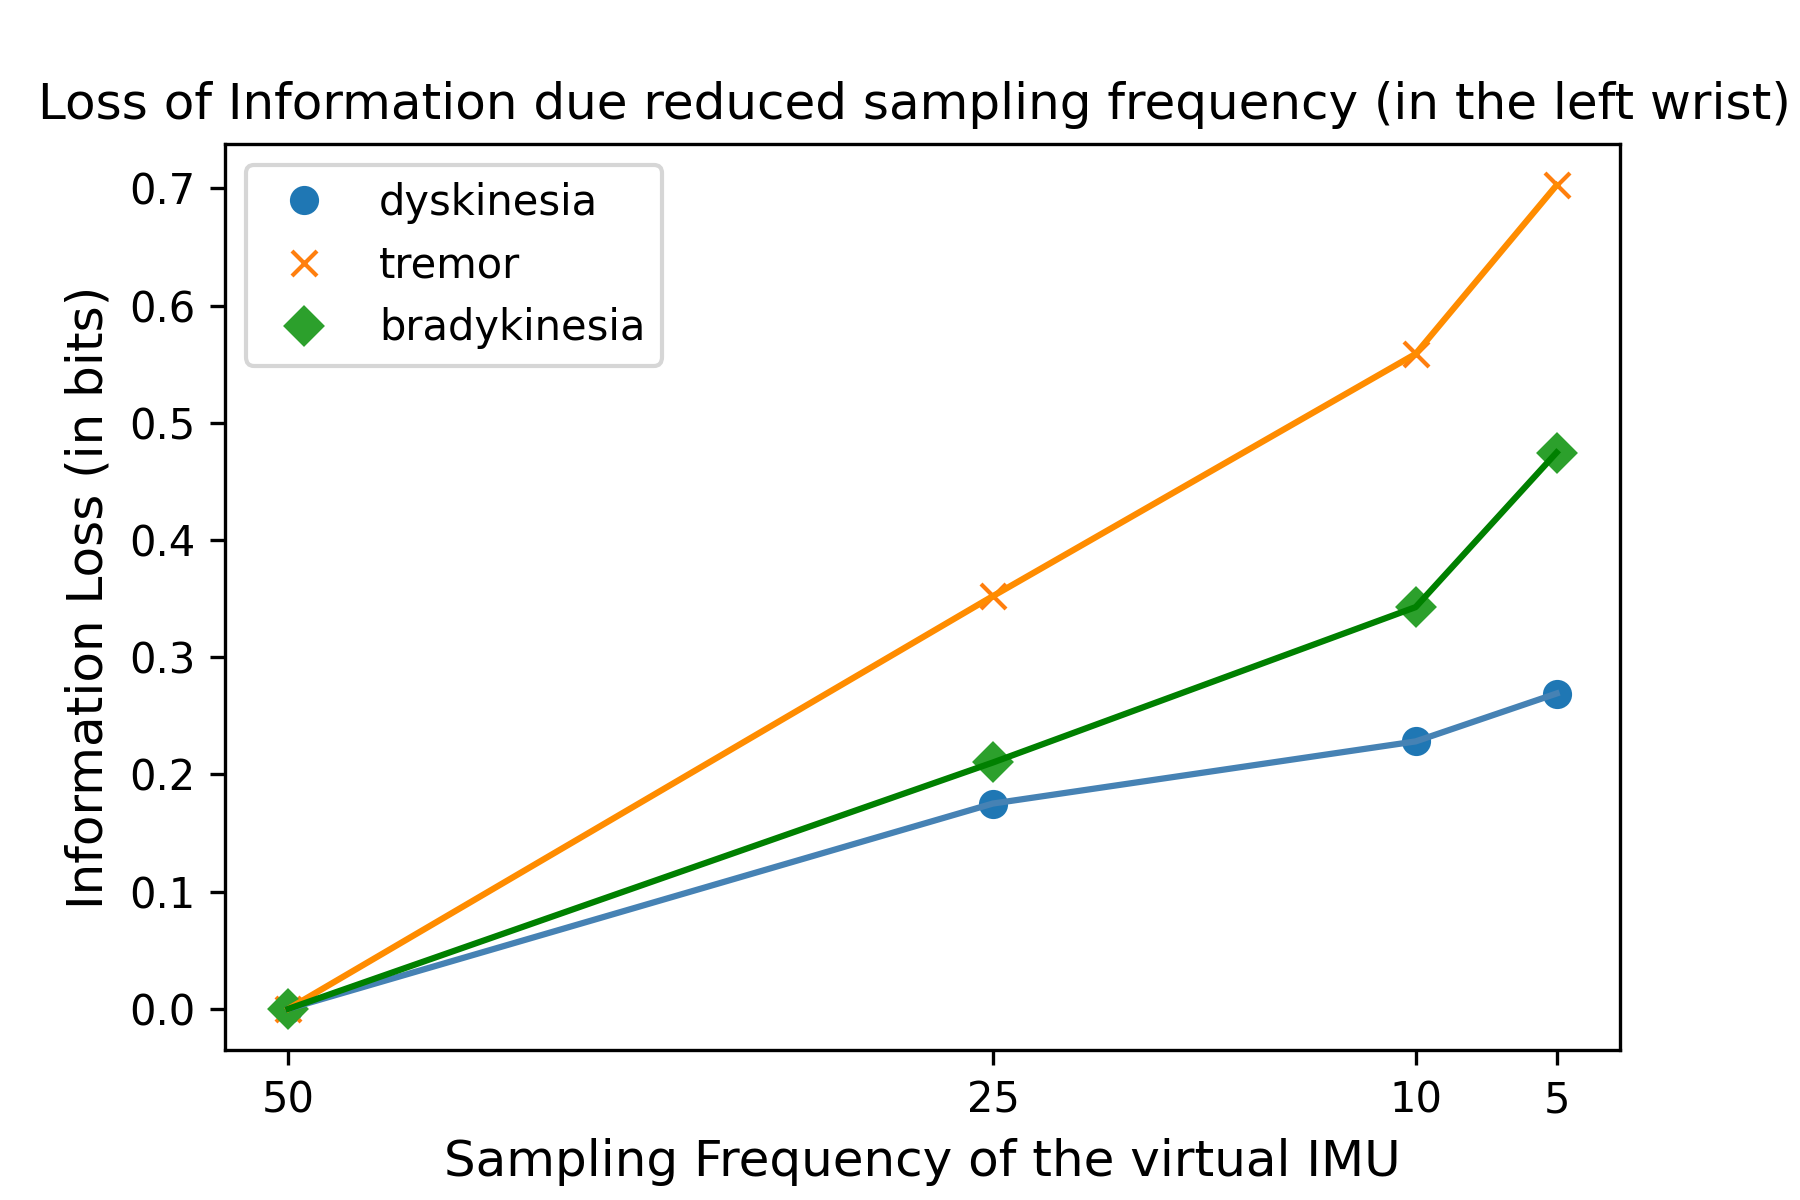
\includegraphics[width=13cm ]{report/pics/7.1.png}
\caption{Variation in information loss with decreasing sampling frequency in patients 3, 6, 7, 9 left wrists under tremor, dyskinesia, and bradykinesia disorders.}
\end{figure} \\

We next proceeded to calculate, for these four patients, the loss of information in the right wrist as the sampling frequency decreased in the three cases. The classification categories for their ratings under the three conditions were the same as for the left wrist.
\begin{figure}[htbp]
\centering
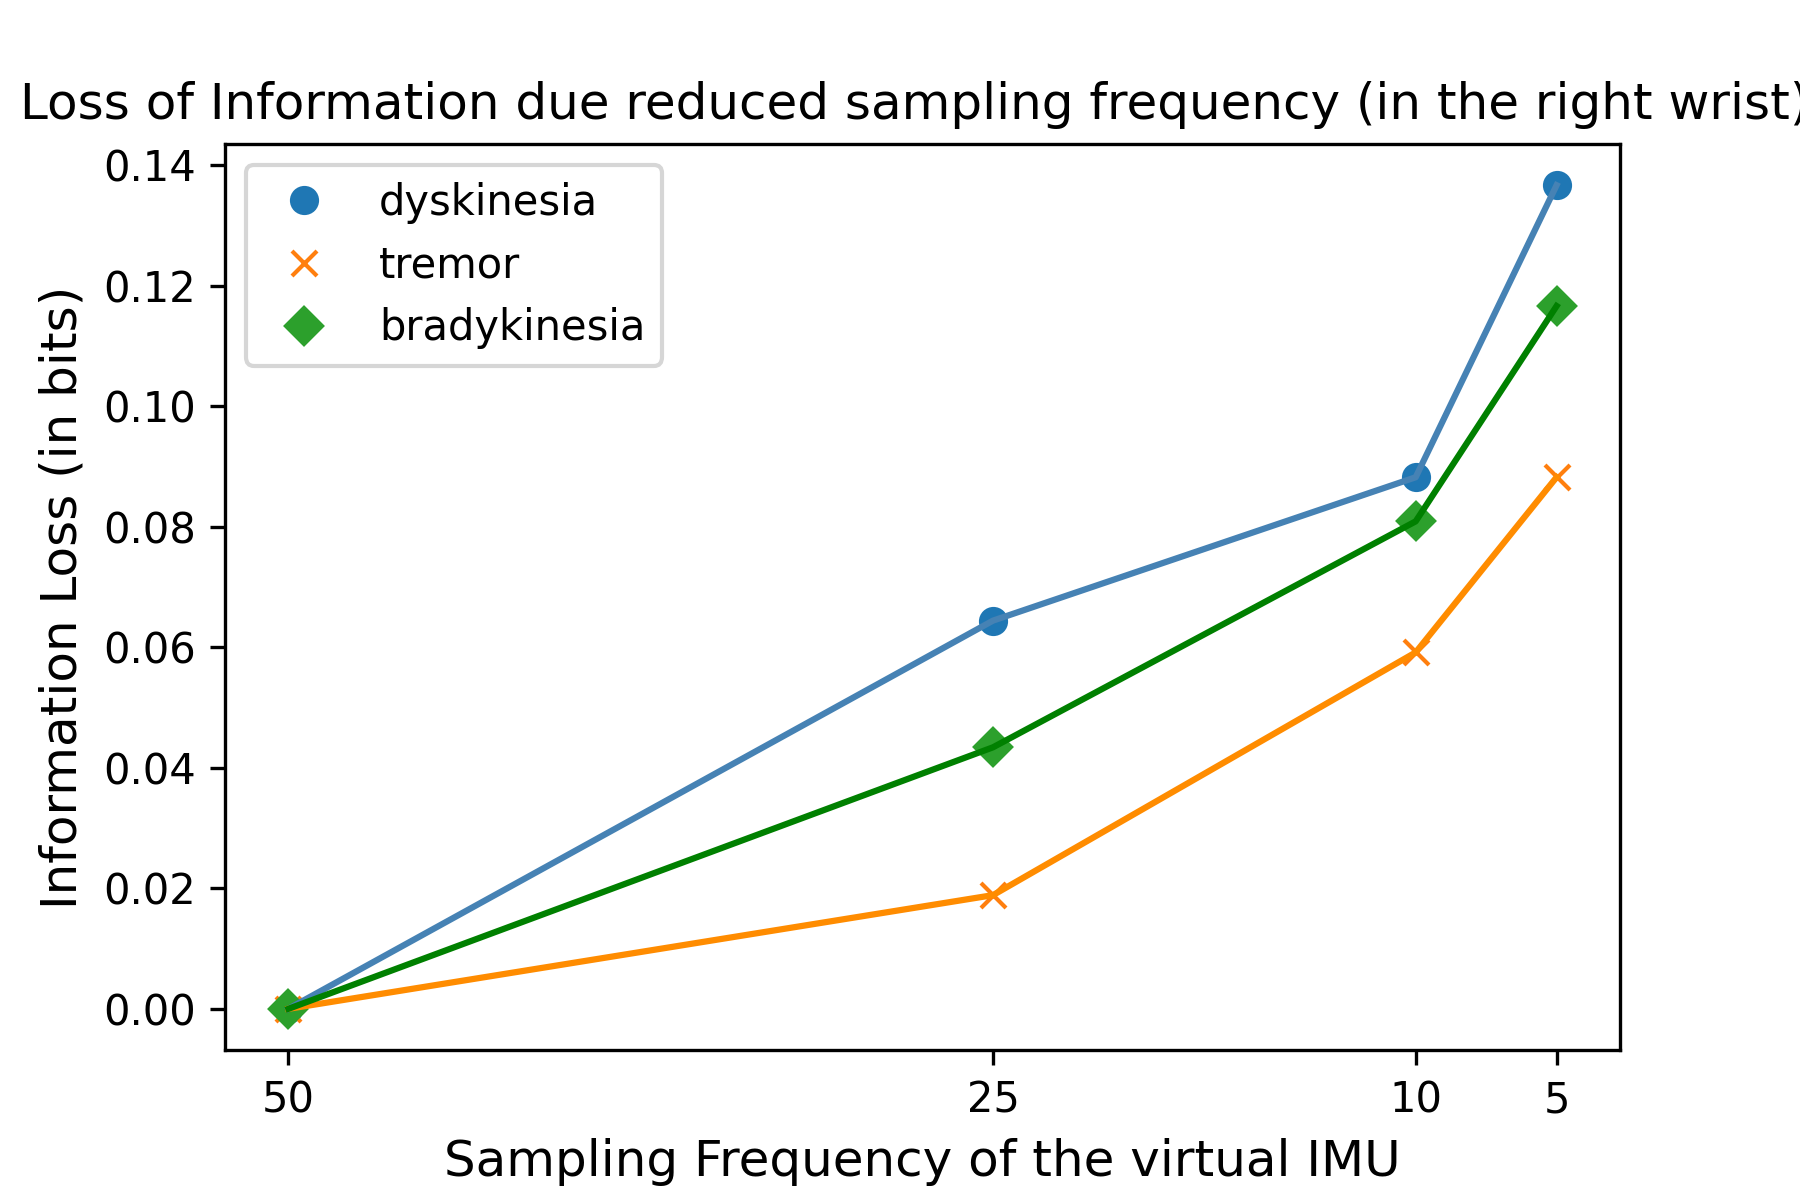
\includegraphics[width=13cm ]{report/pics/7.2.png}
\caption{Variation in information loss with decreasing sampling frequency in patients 3, 6, 7, 9 right wrists under tremor, dyskinesia, and bradykinesia disorders.}
\end{figure}\\
As shown in Figure 7.2, the change in information loss in the patient's right wrist was similar to that in the left wrist in all three conditions, but the information loss in the right wrist was relatively less compared to that in the left wrist.\\

Finally, we calculated the information loss with decreasing sampling frequency for the left ankle of four patients with tremor and dyskinesia. We did not calculate the information loss for bradykinesia because the data sample was unbalanced. There was no "4" in the tremor rating classification, which differs from the left and right wrists.\\
\begin{figure}[htbp]
\centering
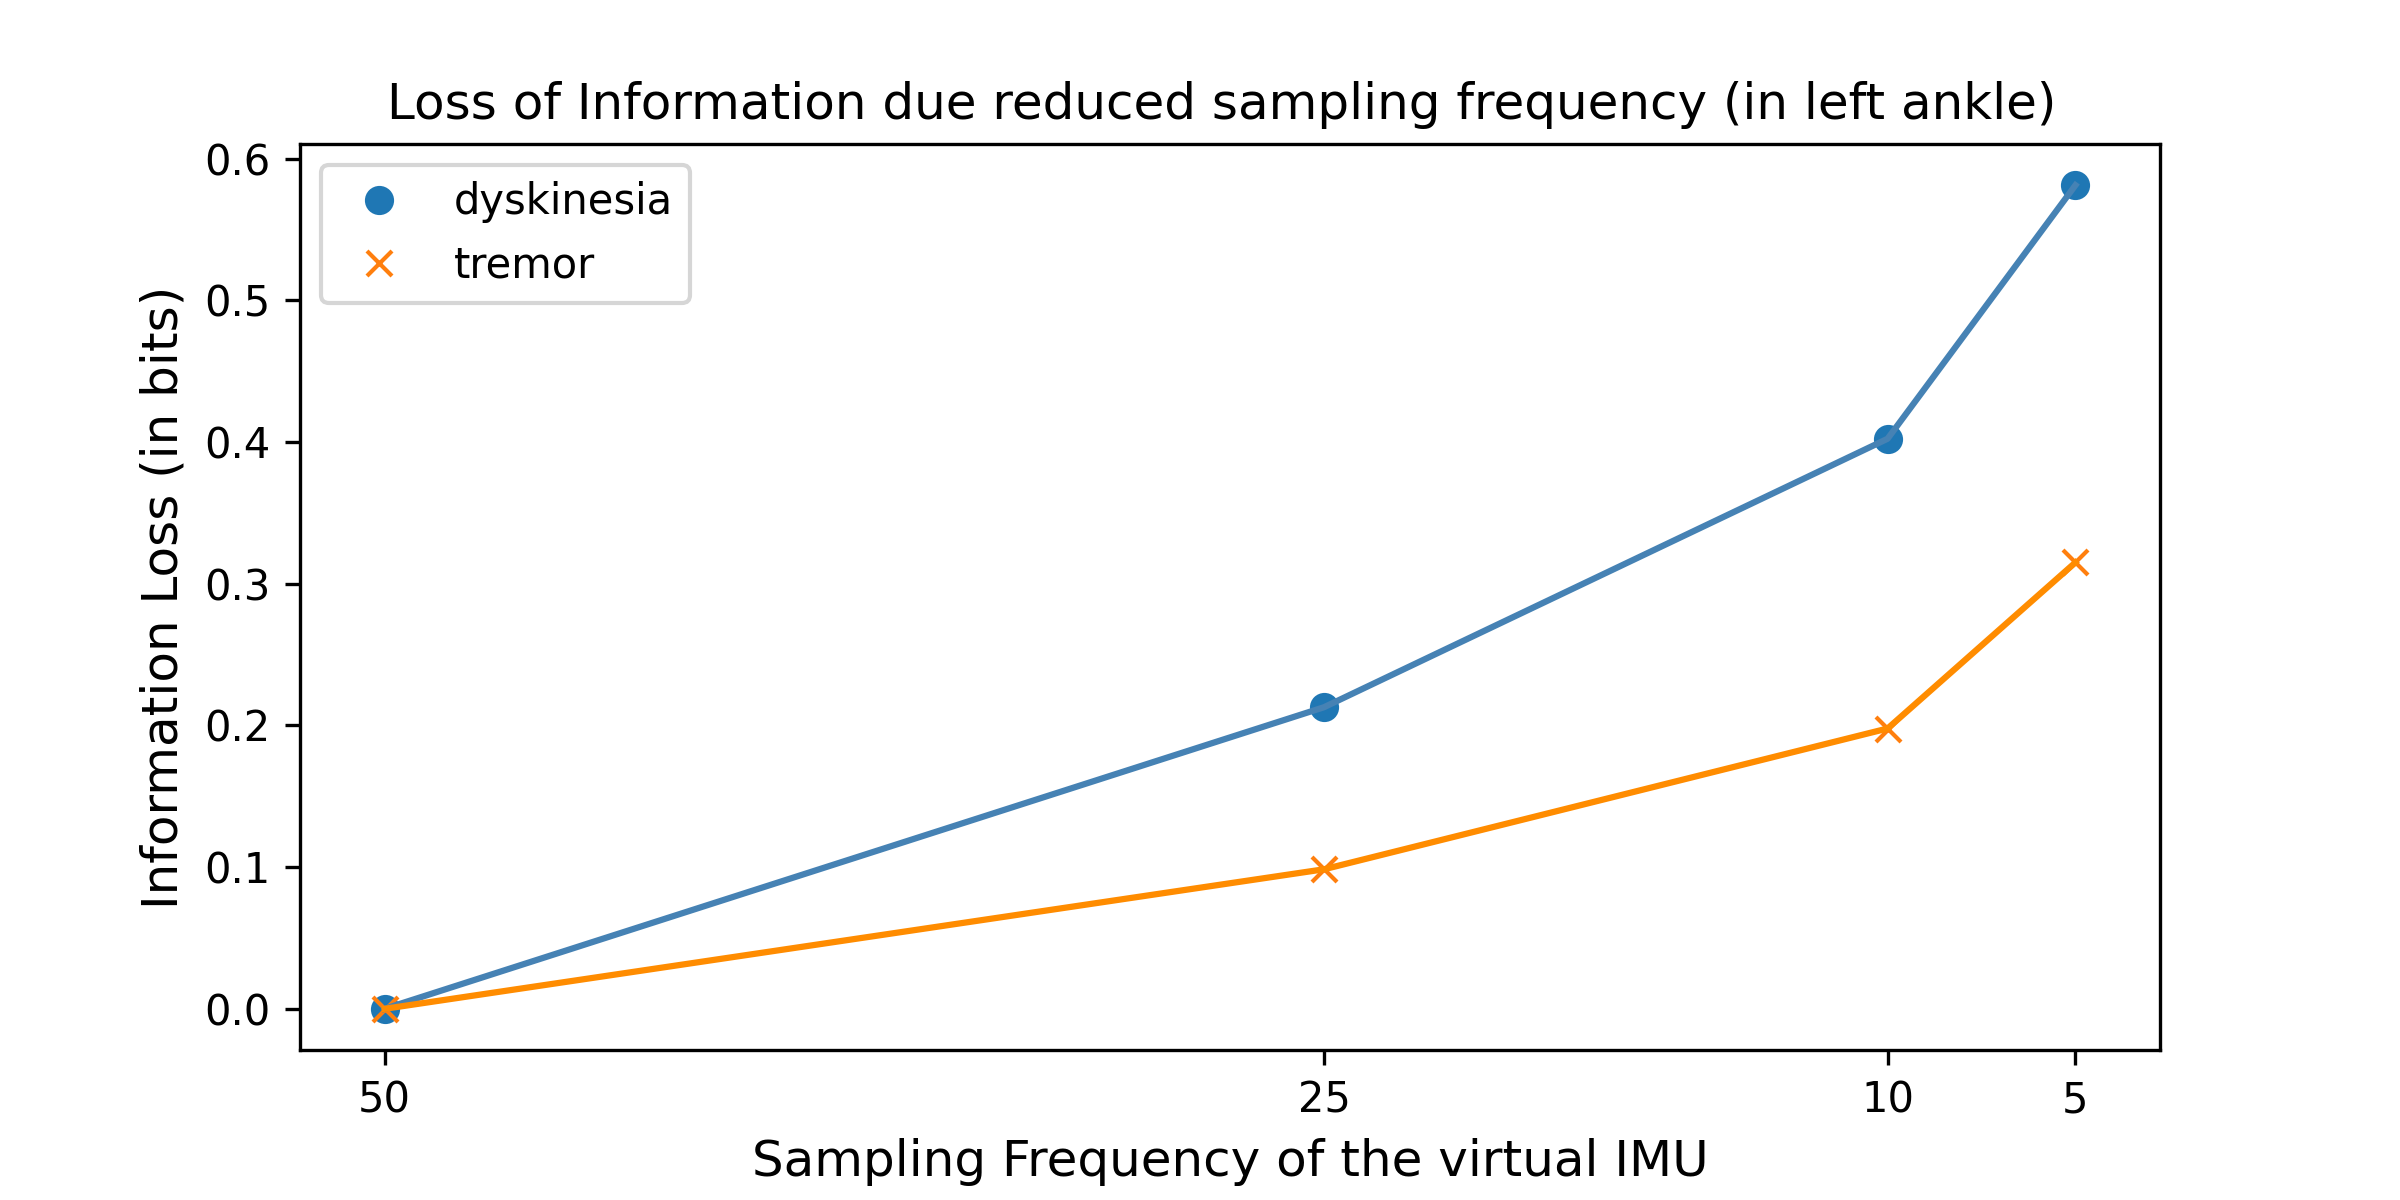
\includegraphics[width=13cm ]{report/pics/7.3.png}
\caption{Variation in information loss with decreasing sampling frequency in patients 3, 6, 7, 9 left ankle under tremor and dyskinesia disorders.}
\end{figure}
As shown in Figure 7.3, the change in information loss is similar for tremor disorders and dyskinesia disorders. However, it is worth noting that the change in information loss for tremor disorder is relatively close when the sampling frequency drops by 25 Hz and 40 Hz. In contrast, the change in information loss for dyskinesia disorder is more pronounced. It is seen that the information loss change is gradually faster in dyskinesia. \\
Combining 7 Fig.1 to 7.3, we can see that the information loss changes under all three disorders are similar at different body parts, with relatively more minor information loss at sampling frequencies down to 25 Hz and some variability at sampling frequencies down to 40 Hz and 45 Hz.


\\ \hspace*{\fill} \\
\section{Results of unbalanced sample data}
In the classification problem with unbalanced data sets, the drawback of KNN is evident, as the minority class is more biased towards the majority class discriminator due to the sample distribution. We can see from the dataset that the severity of Parkinson's disease varies, and typically rating '0' occupies most of the time, while rating '4' does not occupy much time. The sample is unbalanced, increasing our difficulty quantifying the loss of information.\\

\begin{figure}[htbp]
\centering
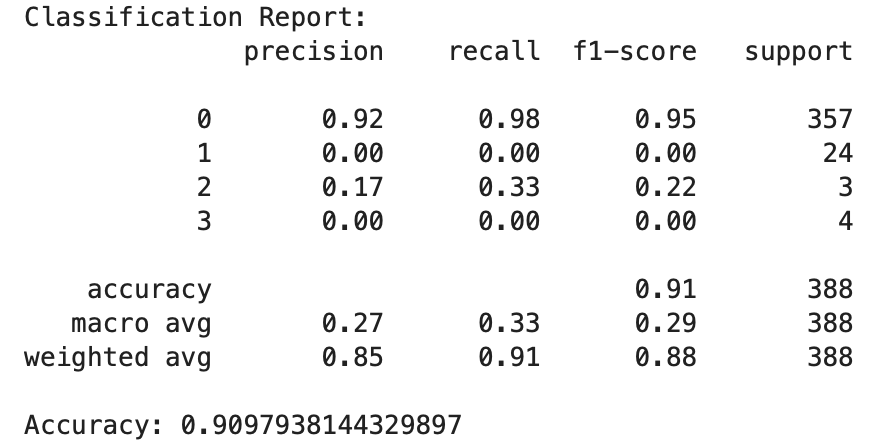
\includegraphics[width=12cm ]{report/chapters/report22.png}
\caption{Patient 9 test set is reported under KNN classification, with different categories corresponding to different data points.}
\end{figure}


\\ \hspace*{\fill} \\
Firstly, we performed KNN classification after classifying the data of patient 9 left wrists under dyskinesia disorder. As shown in Figure 7.4, we have a total of 388 points in our training set, of which class '0': 357 points, class '1': 24 points, class '2' 3 points, and Class '4': 4 points. Such a dataset is unbalanced, and there are far more points in category '0' than in the other categories. kNN classification will incorrectly classify all data points in category 0. Because many categories cannot provide enough training samples, the relatively uniform feature space required by the KNN algorithm cannot be satisfied, making the recognition error larger.\\
We can calculate the information loss when unbalancing the samples and then compare the line plots of information loss. As shown in Figure 7.5, Information loss for patient9 with left wrist dyskinesia disease decreases as the sampling frequency decreases when unbalanced samples are taken.
\begin{figure}[htbp]
\centering
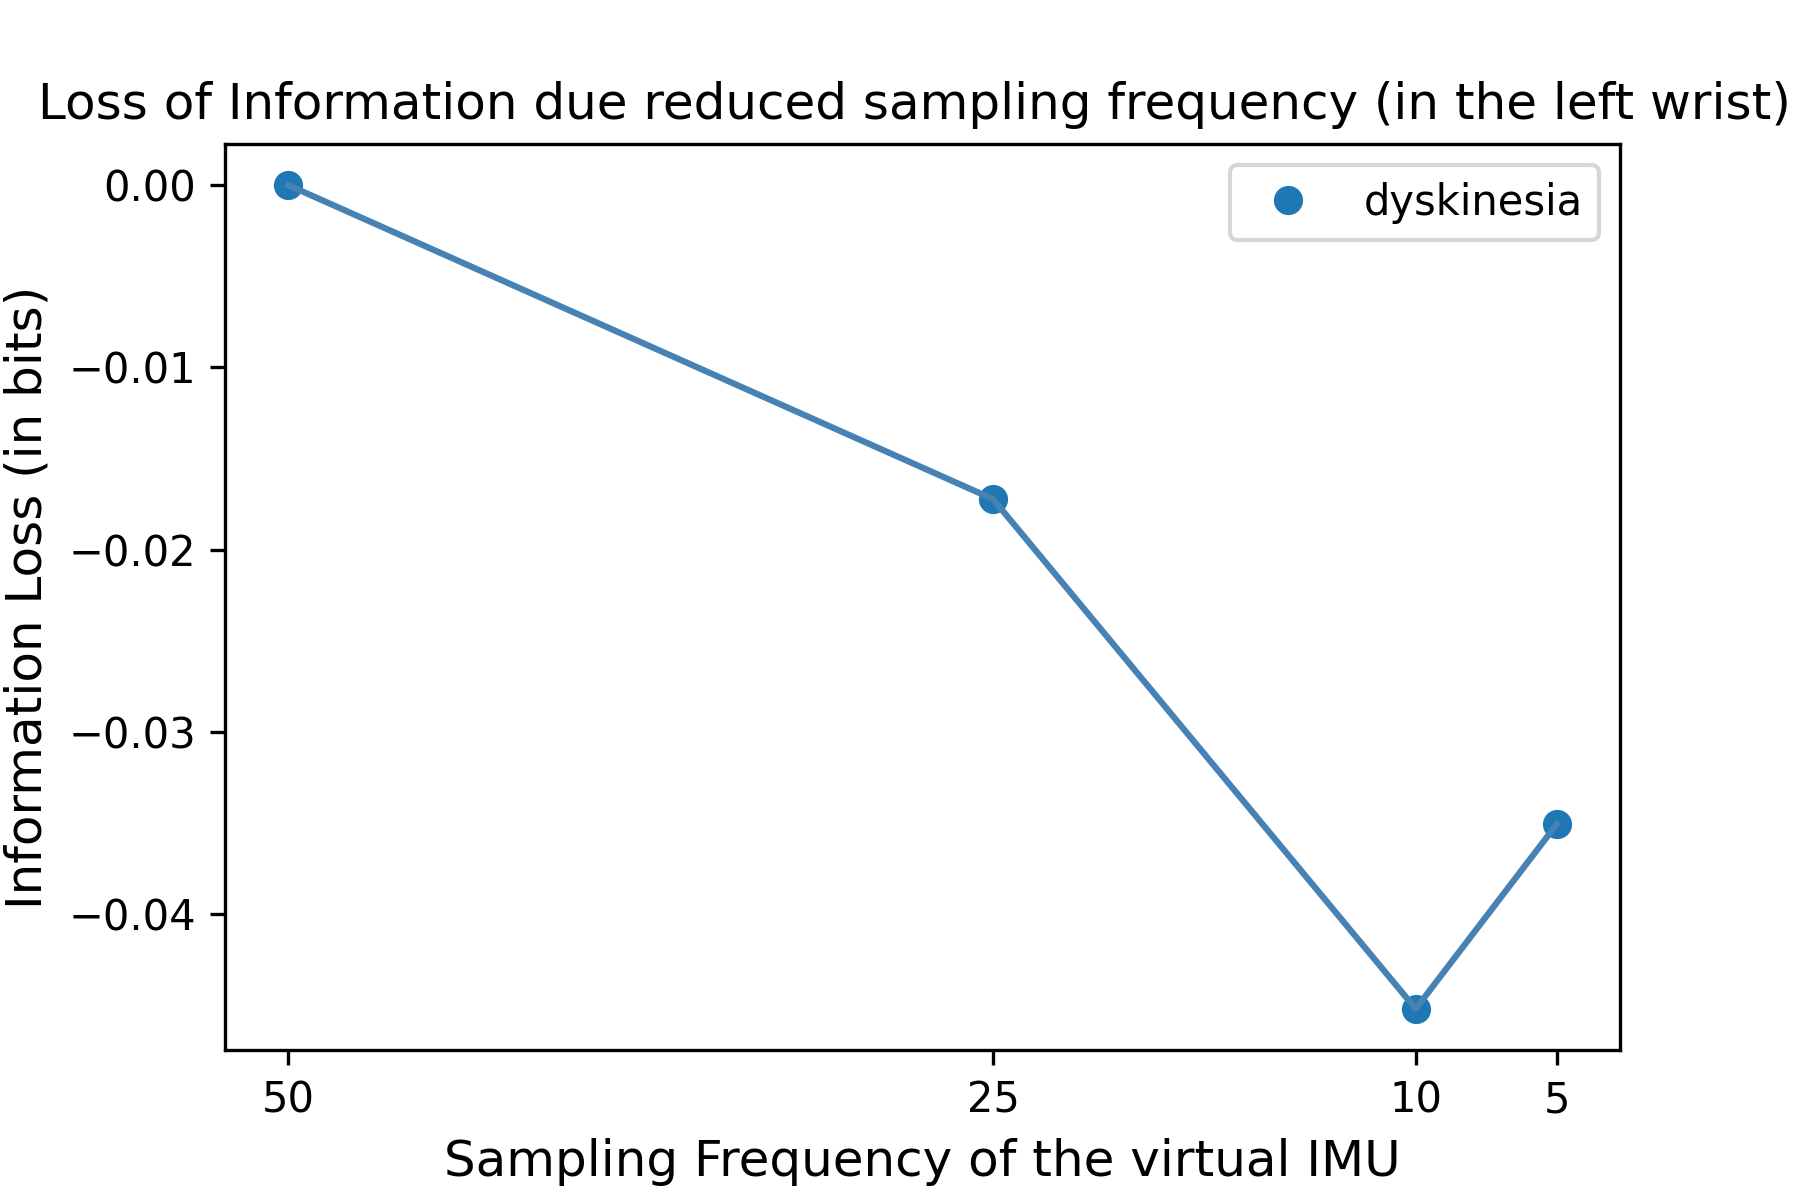
\includegraphics[width=12cm ]{report/pics/dyskinesia_leftwrist9-2.png}
\caption{Information loss with decreasing sampling frequency of IMU sensors in Parkinson's patients9 with left wrist dyskinesia}
\end{figure}\\


As shown in Figure 7.5, we can see a significant error in the information loss and that the information loss is growing inverse. Instead of increasing the information loss, there is a slight decrease; for example, at 25 Hz, there are -0.017 bits of information loss. Such information loss is negligible, and the reason is that most points are classified as '0' during the KNN classification.\\

If our samples are unbalanced, the KNN classification model will learn a priori information about the proportion of samples in the training set. There will be many categories with a focus when predicting with practice. (This may result in better accuracy for the majority category and worse for the minority category.) For example, when the sample size of a category is petite, the probabilities calculated after knn classification are the same as those focused on the majority category, which impacts the calculation of our information loss. To overcome the effect of reducing the sample imbalance KNN classification prediction accuracy, we can weight the categories, for example, use smaller weights for categories with large sample data size. \cite{harrington2012machine} \\
In comparison, we use larger weights for categories with a small sample size. In addition, as the only hyperparameter k of the KNN algorithm, its setting will also significantly impact the algorithm. To reduce the influence of the k value, we can weigh the distance. That is, adding weight to the distance of each point so that the closer points can get a more significant weight. \cite{harrington2012machine}
\\ \hspace*{\fill} \\
Similarly, when calculating the information loss, if there is only one type of classification, the information loss is 0 no matter how to reduce the sampling frequency. Hence, KNN classification is meaningless when there is only one classification category.
\\ \hspace*{\fill} \\
\section{The estimated sampling frequency threshold}
We analyze the calculated information loss results with the differences between categorical categories, Parkinson's disease differences, and where the patient wears the sensor. We could estimate a threshold, the frequency interval where the information loss is minor when the sampling frequency decreases. Our analysis of the information loss plots for the patients showed a similar trend in information loss. When we reduced the sampling frequency to 25 Hz, there was relatively little information loss. However, the information loss increased when we reduced the frequency to 10 Hz and 5 Hz. Comparing the slopes, we conclude that the slopes are relatively small, decreasing in frequency from the original frequency of 50 Hz to 25 Hz. The slope is relatively large, from the original frequency of 50 Hz to the decreasing frequencies of 10 Hz and 5 Hz. therefore, we should choose a frequency between 25 Hz and 50 Hz to obtain a minor information loss at the decreasing frequency. To get a more accurate sampling frequency, we also need to resample the data further and then calculate the information loss. \\
\\ \hspace*{\fill} \\
